%% paper.tex
%% Optimal Retirement Withdrawal Strategies Under Stochastic Returns and Tax Constraints

\documentclass[12pt]{article}

% ── Packages ──────────────────────────────────────────────────────────────────
\usepackage{amsmath, amssymb, amsthm}
\usepackage{booktabs}
\usepackage{array}
\usepackage{graphicx}
\usepackage{caption}
\usepackage[margin=1.25in]{geometry}
\usepackage[colorlinks=true, linkcolor=blue, urlcolor=blue]{hyperref}
\usepackage{setspace}
\usepackage{enumitem}

\onehalfspacing

\newcolumntype{L}[1]{>{\raggedright\arraybackslash}p{#1}}
\newcolumntype{C}[1]{>{\centering\arraybackslash}p{#1}}
\newcolumntype{R}[1]{>{\raggedleft\arraybackslash}p{#1}}

\newtheorem{proposition}{Proposition}
\newtheorem{remark}{Remark}

% ── Notation shorthands ───────────────────────────────────────────────────────
\newcommand{\Tax}{\mathcal{T}}
\newcommand{\Copt}{C^{*}}
\newcommand{\Cmdr}{C^{\mathrm{mrd}}}
\newcommand{\Cdrm}{C^{\mathrm{drm}}}

% ─────────────────────────────────────────────────────────────────────────────
\title{\textbf{Optimal Retirement Withdrawal Strategies Under Stochastic Returns and Tax Constraints}}

\author{Jerry Cubbin\footnote{This paper benefited significantly from working with Claude Code.}}
\date{\today}

\begin{document}
\maketitle
\thispagestyle{empty}

% ── Abstract ──────────────────────────────────────────────────────────────────
\begin{abstract}
We present a framework for choosing annual withdrawals from three retirement
accounts --- a municipal-bond account, a traditional IRA, and a Roth IRA ---
to maximize sustainable after-tax spending over a fixed planning horizon.
Equity returns are stochastic; the municipal-bond rate is deterministic.
Because traditional IRA withdrawals are subject to federal income tax and to
Required Minimum Distributions beginning at age 73, the withdrawal schedule
has both tax and regulatory consequences.
We formulate the single-path problem as a Linear Program (LP) and embed it in a
Monte Carlo simulation over $S = 1{,}000$ independently drawn return sequences.
The optimizer targets a \emph{constant} annual after-tax consumption level
$\Copt$, eliminating year-to-year spending volatility while respecting all
account-balance, tax, and RMD constraints.
Under a representative calibration --- \$500k muni, \$2M traditional IRA,
\$1M Roth, ages 59 to 92 --- the optimizer achieves a median
$\Copt \approx \$258{,}000$ per year, roughly 7\% above the median of two
heuristic benchmark strategies based on fixed account-priority orderings.
Median lifetime federal taxes total approximately \$560k.
\end{abstract}

\newpage
\tableofcontents
\newpage

% =============================================================================
\section{Introduction}
\label{sec:intro}

A retiree who holds wealth across multiple accounts faces a coordination
problem that is easy to understate. The three most common account types ---
a taxable account invested in municipal bonds, a traditional IRA or 401(k),
and a Roth IRA --- differ sharply in their tax treatment:\ municipal-bond
interest is federally tax-free, traditional IRA withdrawals are fully taxable
as ordinary income and subject to Required Minimum Distributions (RMDs)
beginning at age 73, and Roth withdrawals are tax-free with no withdrawal
requirements. The order and timing of withdrawals therefore determines not just
how much is spent each year, but how much of that spending is eroded by taxes
and whether the accounts survive to the planned horizon.

Common practitioner guidance --- deplete taxable accounts first, then the
traditional IRA, then the Roth --- ignores the interaction between withdrawal
timing, marginal tax rates, RMD obligations, and the stochastic growth of
account balances. In good equity markets, the Roth account can grow
dramatically; in bad markets, the traditional IRA may be forced down by RMDs
faster than expected. A strategy that is ``optimal'' on average may perform
poorly on specific return paths, and the only honest assessment is a
distributional one.

This paper develops a computationally tractable framework for the full
three-account problem. The central design choices are as follows.

\begin{enumerate}[leftmargin=2em]
  \item \textbf{Constant consumption.} We maximize $\Copt$, the highest level
        of annual after-tax spending that can be sustained identically in every
        year of the planning horizon. The constant-consumption objective captures
        the preference for smooth spending and produces a single, easily
        interpreted number characterizing each simulated path.

  \item \textbf{Linear Program per path.} For a given realization of stock
        returns, the piecewise-linear tax function makes the withdrawal problem
        a Linear Program (LP) solvable in roughly 25--40\,ms with the
        open-source HiGHS solver. This enables $S = 1{,}000$ Monte Carlo paths
        in under a minute on a standard laptop.

  \item \textbf{Benchmark comparison.} We evaluate the optimizer against two
        ``account-priority'' heuristics --- one drawing the muni account first,
        the other drawing the traditional IRA first --- computed with perfect
        foresight on each realized path via numerical bisection. These
        benchmarks provide a transparent lower bound against which the value
        of joint optimization can be measured.
\end{enumerate}

The remainder of the paper is organized as follows. Section~\ref{sec:model}
develops the model: account dynamics, returns, income, tax, and RMD
constraints. Section~\ref{sec:opt} formulates the optimization problem and
derives the LP reduction. Section~\ref{sec:mc} describes the Monte Carlo
simulation. Section~\ref{sec:benchmarks} defines the benchmark strategies.
Section~\ref{sec:results} presents results under baseline calibration.
Section~\ref{sec:conclusion} concludes with a discussion of extensions.
Appendix~\ref{app:lp} provides the complete LP in standard matrix form;
Appendix~\ref{app:tax} reproduces the 2026 tax schedule;
Appendix~\ref{app:rmd} gives the relevant portion of the IRS Uniform
Lifetime Table.

% =============================================================================
\section{Model}
\label{sec:model}

\subsection{Accounts}
\label{sec:accounts}

An individual of age $a_0$ holds three accounts distinguished by their federal
income tax treatment. Let $t = 0, 1, \ldots, T-1$ index planning years, where
$T = a_\dagger - a_0$ and $a_\dagger$ is the assumed death age. Account balances
$A^j_t$ ($j \in \{m, d, r\}$) are measured at the \emph{start} of year $t$,
before that year's withdrawal.

\begin{itemize}[leftmargin=2em]
  \item \textbf{Municipal-bond account} ($j = m$). A taxable account invested
        in municipal bonds. Federal law exempts muni-bond interest from income
        tax, so both the investment return and withdrawals from this account are
        federally tax-free. The account earns a fixed annual return $r^m$,
        reflecting the predictable nature of investment-grade municipal debt.

  \item \textbf{Traditional IRA / 401(k)} ($j = d$). A tax-\emph{deferred}
        account. Contributions were made pre-tax; every dollar withdrawn is
        treated as ordinary income in the year of withdrawal and taxed
        accordingly. This account is also subject to Required Minimum
        Distributions starting at age $a_{\mathrm{RMD}} = 73$
        (Section~\ref{sec:rmd}).

  \item \textbf{Roth IRA} ($j = r$). A tax-\emph{exempt} account.
        Contributions were made with after-tax dollars; qualified withdrawals
        --- including all investment gains --- are permanently tax-free.
        Unlike the traditional IRA, the Roth carries no RMD requirement during
        the account holder's lifetime, making it the most flexible account from
        a tax-planning standpoint.
\end{itemize}

\subsection{Returns and Account Dynamics}
\label{sec:dynamics}

Each account holds a blend of municipal bonds and equities. Let
$\tilde{r}_t \sim \mathcal{N}(\mu, \sigma^2)$ denote the realized stock
return in year $t$, drawn independently across years. The blended annual
return on account $j$ is
\begin{equation}
  r^j_t \;=\; \alpha_j\,r^m \;+\; (1 - \alpha_j)\,\tilde{r}_t,
  \qquad j \in \{d, r\},
  \label{eq:blended}
\end{equation}
where $\alpha_j \in [0,1]$ is the fraction of account $j$ held in muni bonds.
The muni account itself is entirely in bonds ($\alpha_m = 1$), so its return
$r^m$ is non-stochastic.

Let $w^j_t \geq 0$ denote the withdrawal from account $j$ in year $t$.
Account balances evolve as
\begin{equation}
  A^j_{t+1} \;=\; \bigl(A^j_t - w^j_t\bigr)\bigl(1 + r^j_t\bigr),
  \qquad t = 0, \ldots, T-1,
  \label{eq:dynamics}
\end{equation}
with given initial balances $A^m_0$, $A^d_0$, $A^r_0 \geq 0$.

It is convenient to define cumulative growth factors
\begin{equation}
  G^j_0 = 1, \qquad
  G^j_{t+1} = G^j_t \cdot \bigl(1 + r^j_t\bigr),
  \label{eq:growthfactor}
\end{equation}
so that $G^j_t$ is the factor by which a dollar invested at time 0 in account
$j$ grows by year $t$ (absent any withdrawals). Unrolling
recursion~\eqref{eq:dynamics} gives the closed-form balance
\begin{equation}
  A^j_t \;=\; A^j_0\,G^j_t
          \;-\; \sum_{\tau=0}^{t-1} w^j_\tau \cdot \frac{G^j_t}{G^j_\tau},
  \label{eq:balance_lp}
\end{equation}
which expresses $A^j_t$ as a linear function of the withdrawal history
$\{w^j_0, \ldots, w^j_{t-1}\}$. This linearity is the key structural property
exploited in the LP formulation (Section~\ref{sec:lp}).

\subsection{Income}
\label{sec:income}

Beyond account withdrawals, the individual receives Social Security benefits,
may earn employment income before retirement, and may receive pension income:
\begin{align}
  y^{SS}_t    &= \bar{y}^{SS} \cdot \mathbf{1}\bigl[a_0 + t \geq a_{SS}\bigr],
  \label{eq:ss} \\
  y^{emp}_t   &= \bar{y}^{emp} \cdot \mathbf{1}\bigl[a_0 + t < a_{\mathrm{ret}}\bigr],
  \label{eq:emp} \\
  y^{pen}_t   &= \bar{y}^{pen} \cdot \mathbf{1}\bigl[a_0 + t \geq a_{\mathrm{ret}}\bigr],
  \label{eq:pen}
\end{align}
where $\bar{y}^{SS}$ is the elected annual Social Security benefit, $a_{SS}$
is the claiming age, $\bar{y}^{emp}$ is annual pre-retirement earned income,
$\bar{y}^{pen}$ is the annual pension benefit, and $a_{\mathrm{ret}}$ is the age
at which employment income ceases and pension income begins.
Social Security income is partially taxable ($\phi = 0.85$); employment and pension income are fully taxable.
Municipal-bond interest and Roth withdrawals are excluded from ordinary income. The taxable ordinary
income in year $t$ is therefore
\begin{equation}
  I_t \;=\; w^d_t + \phi\,y^{SS}_t + y^{emp}_t + y^{pen}_t.
  \label{eq:income}
\end{equation}
Pension income $y^{pen}_t$ is fully included in ordinary income beginning at
retirement age; setting $\bar{y}^{pen} = 0$ recovers the no-pension baseline.


\subsection{Federal Income Tax}
\label{sec:tax}

We model federal income tax under the 2026 Married Filing Jointly (MFJ)
brackets, reproduced in Appendix~\ref{app:tax}. The annual tax liability is
computed after applying the standard deduction $\Delta$:\ taxable income
equals $\max(0,\, I_t - \Delta)$.

With $K$ brackets having lower bounds $L_k$ and marginal rates
$\tau_0 < \tau_1 < \cdots < \tau_{K-1}$, the tax function can be written as
\begin{equation}
  \Tax(I) \;=\; \sum_{k=0}^{K-1} \Delta\tau_k \cdot \max\!\bigl(0,\;
                I - \Delta - L_k\bigr),
  \label{eq:tax}
\end{equation}
where $\Delta\tau_k = \tau_k - \tau_{k-1}$ (with $\tau_{-1} \equiv 0$) is the
incremental rate at each bracket threshold. This \emph{incremental-rate}
formulation decomposes the tax calculation into $K$ separate
``income above threshold'' terms, each individually convex and non-decreasing.
The function $\Tax(I)$ is piecewise linear, convex, and continuous.

\begin{remark}
  The incremental-rate formula~\eqref{eq:tax} is algebraically equivalent to
  the standard ``fill from the bottom'' bracket calculation.  Its value for
  our purposes is that each $\max(0, \cdot)$ term can be replaced by a
  non-negative slack variable in the LP, yielding a fully linear model
  (Section~\ref{sec:lp}).
\end{remark}

\subsection{Required Minimum Distributions}
\label{sec:rmd}

Federal law requires holders of traditional IRA and 401(k) accounts to
withdraw a minimum amount each year beginning at age $a_{\mathrm{RMD}} = 73$.
The Required Minimum Distribution (RMD) is calculated by dividing the
account balance by the IRS Uniform Lifetime Table distribution period $\nu_t$,
which depends on the account holder's age (Appendix~\ref{app:rmd}):
\begin{equation}
  \rho_t \;=\; \frac{A^d_t}{\nu_t}.
  \label{eq:rmd_amount}
\end{equation}
The RMD imposes a lower bound on traditional IRA withdrawals:
\begin{equation}
  w^d_t \;\geq\; \rho_t \;=\; \frac{A^d_t}{\nu_t},
  \qquad \text{for } a_0 + t \geq a_{\mathrm{RMD}}.
  \label{eq:rmd}
\end{equation}
Roth accounts are not subject to RMD requirements.

Two features of the RMD constraint are worth noting. First, because $A^d_t$
depends on prior withdrawals, the constraint is not a simple lower bound on
$w^d_t$ in isolation; it couples the decision variables across time in a way
that must be handled carefully in the LP (Section~\ref{sec:lp}). Second,
since the distribution period $\nu_t$ declines with age, the required
fraction of the account that must be distributed rises over time, from
roughly 3.8\% at age 73 to over 8\% by age 90.

\subsection{Early Withdrawal Penalty}
\label{sec:penalty}

Federal law imposes a 10\% penalty on traditional IRA distributions taken
before the account holder reaches age $59\tfrac{1}{2}$. Defining the
per-year penalty rate
\begin{equation}
  \pi_t \;=\; \begin{cases} 0.10 & \text{if } a_0 + t < 59.5, \\
                             0   & \text{otherwise,} \end{cases}
  \label{eq:penalty_rate}
\end{equation}
the total tax and penalty burden on traditional IRA withdrawals in year $t$
is $\Tax(I_t) + \pi_t\,w^d_t$.

Because $\pi_t\,w^d_t$ is already linear in the decision variable $w^d_t$,
the penalty integrates into the LP without introducing any new variables or
constraints: it simply reduces the net consumption coefficient on $w^d_t$
from 1 to $(1 - \pi_t)$ in the constant-consumption equality rows
(Section~\ref{sec:lp}).  The optimizer therefore automatically avoids
traditional IRA withdrawals in penalty-eligible years, preferring tax-free
muni and Roth draws instead.

% =============================================================================
\section{Optimization Problem}
\label{sec:opt}

\subsection{Objective: Maximum Constant Consumption}
\label{sec:objective}

After-tax consumption in year $t$ is total income from all sources minus
federal income tax and any early withdrawal penalty:
\begin{equation}
  c_t \;=\; w^m_t + w^d_t + w^r_t + y^{SS}_t + y^{emp}_t + y^{pen}_t
           - \Tax(I_t) - \pi_t\,w^d_t,
  \label{eq:consumption}
\end{equation}
where $\pi_t$ is defined in~\eqref{eq:penalty_rate}. Equivalently,
$c_t = w^m_t + (1-\pi_t)\,w^d_t + w^r_t + y^{SS}_t + y^{emp}_t + y^{pen}_t - \Tax(I_t)$.
Our primary objective is to find withdrawal schedules
$\{w^m_t, w^d_t, w^r_t\}_{t=0}^{T-1}$ that maximize a constant annual
after-tax consumption level $\Copt$ subject to $c_t = \Copt$ for every
year $t$. In other words, we look for the highest sustainable flat spending
rate over the entire planning horizon.

The constant-consumption objective has several practical advantages.  It
directly quantifies the ``permanent income'' the portfolio can support,
yielding a single scalar $\Copt$ that is easy to interpret and compare
across simulations.  It also eliminates the need to specify a discount rate
or utility function: maximizing the level of a permanently flat consumption
stream requires no preference assumptions beyond the preference for more over
less.

\subsection{Constraints}
\label{sec:constraints}

For a given realized return path $\{\tilde{r}_t\}_{t=0}^{T-1}$, the
optimization problem is subject to the following constraints.

\begin{enumerate}[label=(\roman*), leftmargin=2em]
  \item \textbf{Non-negative withdrawals.}
        $w^j_t \geq 0$ for all $j \in \{m, d, r\}$ and $t = 0, \ldots, T-1$.
        Withdrawals cannot be negative; re-contribution of funds is not modeled.

  \item \textbf{Non-negative account balances.}
        $A^j_t \geq 0$ for all $j$ and $t = 1, \ldots, T$. An account
        cannot be overdrawn. Using representation~\eqref{eq:balance_lp},
        this condition becomes a set of linear inequalities in the withdrawal
        history up to time $t$.

  \item \textbf{RMD constraint.}
        Substituting the closed-form expression~\eqref{eq:balance_lp} for
        $A^d_t$ into constraint~\eqref{eq:rmd} gives
        \begin{equation}
          \nu_t\,w^d_t + \sum_{\tau=0}^{t-1} w^d_\tau \cdot
          \frac{G^d_t}{G^d_\tau}
          \;\geq\; A^d_0\,G^d_t,
          \qquad a_0 + t \geq a_{\mathrm{RMD}},
          \label{eq:rmd_lp}
        \end{equation}
        which is linear in the withdrawal variables.

  \item \textbf{Constant consumption.}
        $c_t = \Copt$ for all $t = 0, \ldots, T-1$, where $\Copt$ is treated
        as a scalar decision variable to be maximized. After the tax
        linearization described in Section~\ref{sec:lp}, this yields $T$
        linear equality constraints.
\end{enumerate}

\begin{remark}[Terminal balances and feasibility]
  \label{rem:terminal}
  We do \emph{not} impose terminal equality constraints $A^j_T = 0$.
  The balance non-negativity constraints already enforce $A^j_T \geq 0$,
  and the maximize-$\Copt$ objective naturally pushes all three accounts
  toward zero by incentivizing higher withdrawals throughout the horizon.
  In practice, the muni and traditional accounts are depleted to zero in
  the large majority of simulations.

  The Roth account, held entirely in equities, can grow faster than the
  constant-consumption constraint allows it to be drawn down --- particularly
  in Social Security years when SS income already covers most of $\Copt$,
  leaving little room for additional Roth withdrawals without exceeding $\Copt$.
  On such paths, a small positive Roth balance remains at death: an
  unintended bequest rather than an infeasibility.

  Imposing a terminal equality $A^j_T = 0$ instead would render these
  extreme paths infeasible with no optimal solution. The inequality
  formulation is always feasible.
\end{remark}

\subsection{LP Reformulation}
\label{sec:lp}

The tax function $\Tax(I_t)$ in constraint~(iv) is piecewise linear and
convex, so it cannot appear directly in an LP. We handle it by introducing
\emph{bracket slack variables} $s_{tk} \geq 0$ defined to satisfy
\begin{equation}
  s_{tk} \;=\; \max\!\bigl(0,\; I_t - \Delta - L_k\bigr)
         \;=\; \max\!\bigl(0,\; w^d_t + \phi\,y^{SS}_t + y^{emp}_t + y^{pen}_t - \Delta - L_k\bigr).
  \label{eq:slack_def}
\end{equation}
With this definition, the tax on year-$t$ income is exactly
\begin{equation}
  \Tax(I_t) \;=\; \sum_{k=0}^{K-1} \Delta\tau_k \cdot s_{tk},
  \label{eq:tax_lp}
\end{equation}
which is linear in the slack variables. The constraint
$s_{tk} \geq I_t - \Delta - L_k$ is imposed as the LP inequality
\begin{equation}
  w^d_t - s_{tk} \;\leq\; \Delta + L_k - \phi\,y^{SS}_t - y^{emp}_t - y^{pen}_t,
  \qquad t = 0,\ldots,T-1,\; k = 0,\ldots,K-1.
  \label{eq:slack_ineq}
\end{equation}
Because the LP objective drives $s_{tk}$ to its minimum feasible value
(higher slacks represent higher taxes, which reduce the consumption that
can be achieved), the slacks will equal exactly the quantities in
\eqref{eq:slack_def} at any optimal solution.

Substituting~\eqref{eq:tax_lp} into the constant-consumption condition
$c_t = \Copt$ and rearranging using~\eqref{eq:consumption} yields
\begin{equation}
  w^m_t + (1-\pi_t)\,w^d_t + w^r_t
  - \sum_{k=0}^{K-1} \Delta\tau_k\, s_{tk} - \Copt
  \;=\; -y^{SS}_t - y^{emp}_t - y^{pen}_t,
  \qquad t = 0,\ldots,T-1,
  \label{eq:cc_lp}
\end{equation}
which is a system of $T$ linear equalities in the decision variables.
The coefficient $(1-\pi_t)$ on $w^d_t$ reflects the early withdrawal penalty:
in years before age $59\tfrac{1}{2}$ only 90\% of each traditional IRA dollar
withdrawn reaches after-tax consumption.

\begin{proposition}
  The optimal withdrawal problem is a Linear Program in the
  $N + 1 = 3T + TK + 1$ variables
  \[
    \bigl(\,w^m_0,\ldots,w^m_{T-1},\;\;
          w^d_0,\ldots,w^d_{T-1},\;\;
          w^r_0,\ldots,w^r_{T-1},\;\;
          \{s_{tk}\},\;\;
          \Copt\,\bigr),
  \]
  with objective $\min\; -\Copt$, subject to the linear constraints
  \eqref{eq:slack_ineq} and \eqref{eq:cc_lp}, the balance non-negativity
  constraints derived from~\eqref{eq:balance_lp}, the RMD constraints
  \eqref{eq:rmd_lp}, and the non-negativity of all withdrawal and slack
  variables. The variable $\Copt$ is unrestricted in sign.
\end{proposition}

Appendix~\ref{app:lp} presents the full LP in standard matrix form.
Under baseline calibration ($T = 33$, $K = 7$) the LP has $3(33) + 33(7) + 1
= 331$ variables and approximately 600 constraints, and is solved in
25--40\,ms by HiGHS.

% =============================================================================
\section{Monte Carlo Simulation}
\label{sec:mc}

For each simulation $s = 1, \ldots, S$, we independently draw a $T$-year
stock-return sequence $\{\tilde{r}^{(s)}_t\}_{t=0}^{T-1}$, with each
$\tilde{r}^{(s)}_t \sim \mathcal{N}(\mu, \sigma^2)$. All paths use the same
mean $\mu$ and volatility $\sigma$; the randomness enters only through the
realized draws. A fixed random seed is used to ensure reproducibility.

For each path we:
\begin{enumerate}[leftmargin=2em]
  \item Compute the blended returns $r^d_t$ and $r^r_t$ and their cumulative
        growth factors $G^d_t$ and $G^r_t$ (the muni growth factors $G^m_t$
        are path-independent).
  \item Construct the LP described in Section~\ref{sec:lp}.
  \item Solve the LP to obtain the optimal withdrawals
        $\{w^{m*}_t, w^{d*}_t, w^{r*}_t\}$ and constant consumption $C^{*(s)}$.
  \item Compute account balance paths $A^j_t$, taxes $\Tax(I_t)$,
        and effective marginal rates from the solution.
  \item Compute both benchmark consumption levels $C^{\mathrm{mrd}(s)}$ and
        $C^{\mathrm{drm}(s)}$ by bisection (Section~\ref{sec:benchmarks}).
\end{enumerate}

All results are stored in a long-format panel indexed by $(s, t)$ and
summarized across simulations by quantiles of $C^{*(s)}$, lifetime taxes
$\sum_t \Tax(I^{(s)}_t)$, and account balance trajectories.

% =============================================================================
\section{Benchmark Strategies}
\label{sec:benchmarks}

To assess the value of joint optimization, we compare $\Copt$ against two
heuristic strategies that observe the same realized return path but follow a
fixed account-priority ordering rather than solving an LP.

\subsubsection*{Muni-first (\texorpdfstring{$\Cmdr$}{C-mdr}):
  $A^m \to A^r \to A^d$}

Draw first from the municipal-bond account until it is exhausted, then from
the Roth, then from the traditional IRA. In each year, the withdrawal from
the currently active account is the minimum needed to reach the target
consumption $C$, netting any taxes owed on the traditional IRA portion. The
ordering was chosen to defer taxable income as long as possible, letting
the tax-deferred and Roth accounts compound on a larger base.

Given a realized path, the maximum sustainable constant consumption under
this ordering is found by bisection: increase $C$ until the terminal
balance of the last account (traditional IRA) transitions from positive
to negative, then recover the zero-crossing by Brent's method.

\subsubsection*{Deferred-first (\texorpdfstring{$\Cdrm$}{C-drm}):
  $A^d \to A^r \to A^m$}

Draw first from the traditional IRA until exhausted, then the Roth, then
the muni account. This front-loads the tax burden but leaves the tax-free
accounts to grow for longer. The same bisection procedure is applied, with
the terminal muni-account balance as the target function.

\subsubsection*{Properties of the benchmarks}

Both strategies are always feasible (account balances are floored at zero
rather than required to hit exactly zero), and both use perfect foresight
over the realized return path. The optimizer has strictly more freedom: it
can mix withdrawals across accounts in any year, is not constrained to a
priority ordering, and jointly optimizes the tax consequences of all
decisions. Therefore $C^{*(s)} \geq \max(C^{\mathrm{mrd}(s)}, C^{\mathrm{drm}(s)})$
for every path $s$, and the gap between $\Copt$ and the benchmarks measures
the value of joint optimization relative to the best simple heuristic.

% =============================================================================
\section{Results}
\label{sec:results}

\subsection{Baseline Calibration}

Table~\ref{tab:params} summarizes the parameters used in the baseline
simulation. The planning horizon spans $T = 33$ years (ages 59--91).
The individual has no employment income ($\bar{y}^{emp} = 0$), retires at
age 65 (though this has no effect in the baseline since $\bar{y}^{emp} = 0$),
claims Social Security at age 70, and faces RMDs from age 73 onward.
The Roth is held entirely in equities ($\alpha_r = 0$) to maximize
tax-free compounding; the traditional IRA holds a 40\% muni bond position
($\alpha_d = 0.40$) to moderate volatility on the taxable account.
All 1,000 simulated paths are solved to optimality.

\begin{table}[h]
\centering
\caption{Baseline Parameters}
\label{tab:params}
\begin{tabular}{@{} L{5.5cm} C{2cm} C{3cm} @{}}
\toprule
\textbf{Parameter} & \textbf{Symbol} & \textbf{Value} \\
\midrule
\multicolumn{3}{@{}l}{\textit{Ages}} \\
Start age            & $a_0$              & 59 \\
Retirement age       & $a_{\mathrm{ret}}$ & 65 \\
Social Security age  & $a_{SS}$           & 70 \\
RMD start age        & $a_{\mathrm{RMD}}$ & 73 \\
Death age            & $a_\dagger$        & 92 \\[4pt]
\multicolumn{3}{@{}l}{\textit{Initial account balances}} \\
Municipal-bond account & $A^m_0$ & \$500,000 \\
Traditional IRA        & $A^d_0$ & \$2,000,000 \\
Roth IRA               & $A^r_0$ & \$1,000,000 \\[4pt]
\multicolumn{3}{@{}l}{\textit{Asset allocation (muni fraction)}} \\
Traditional IRA  & $\alpha_d$ & 40\% \\
Roth IRA         & $\alpha_r$ & 0\% \\[4pt]
\multicolumn{3}{@{}l}{\textit{Investment returns}} \\
Municipal-bond rate & $r^m$ & 3.0\% \\
Stock mean return   & $\mu$   & 7.0\% \\
Stock volatility    & $\sigma$ & 15.0\% \\[4pt]
\multicolumn{3}{@{}l}{\textit{Social Security}} \\
Annual benefit   & $\bar{y}^{SS}$ & \$120,000 \\
Taxable fraction & $\phi$         & 85\% \\[4pt]
\multicolumn{3}{@{}l}{\textit{Simulation}} \\
Number of paths & $S$ & 1,000 \\
Tax schedule    &     & 2026 MFJ (Appendix~\ref{app:tax}) \\
\bottomrule
\end{tabular}
\end{table}

\subsection{Consumption Outcomes}

Table~\ref{tab:consumption} reports the cross-simulation distribution of
annual after-tax consumption under the optimizer and the two benchmarks.

\begin{table}[h]
\centering
\caption{Distribution of Annual After-Tax Consumption Across 1,000 Simulations (\$)}
\label{tab:consumption}
\begin{tabular}{@{} L{5.5cm} rrrrr @{}}
\toprule
\textbf{Strategy} & \textbf{P10} & \textbf{P25} & \textbf{Median} & \textbf{P75} & \textbf{P90} \\
\midrule
Optimizer ($\Copt$)       & 211,803 & 230,654 & 258,249 & 294,341 & 336,231 \\
Muni-first ($\Cmdr$)      & 197,900 & 216,148 & 242,254 & 270,799 & 301,866 \\
Deferred-first ($\Cdrm$)  & 195,588 & 213,816 & 238,590 & 268,612 & 302,104 \\
\bottomrule
\end{tabular}
\end{table}

The optimizer achieves a median constant consumption of \$258,249 per year,
approximately 6.6\% above the muni-first benchmark (\$242,254) and 8.2\%
above the deferred-first benchmark (\$238,590). The improvement arises from
the optimizer's ability to blend withdrawals across accounts in every year to
keep the traditional IRA's marginal contribution to taxable income within
lower brackets. In particular, the optimizer draws more heavily from the
traditional IRA in pre-Social Security years (ages 59--69), when $I_t = w^d_t$
alone and the standard deduction absorbs the first \$32,200 of income,
then draws more from the tax-free muni and Roth accounts in later years when
Social Security adds \$102,000 of taxable income. The fixed-ordering heuristics
cannot make this intertemporal adjustment.

Figure~\ref{fig:consumption} shows the distributional comparison between the
optimizer and the two benchmarks.

\begin{figure}[h]
  \centering
  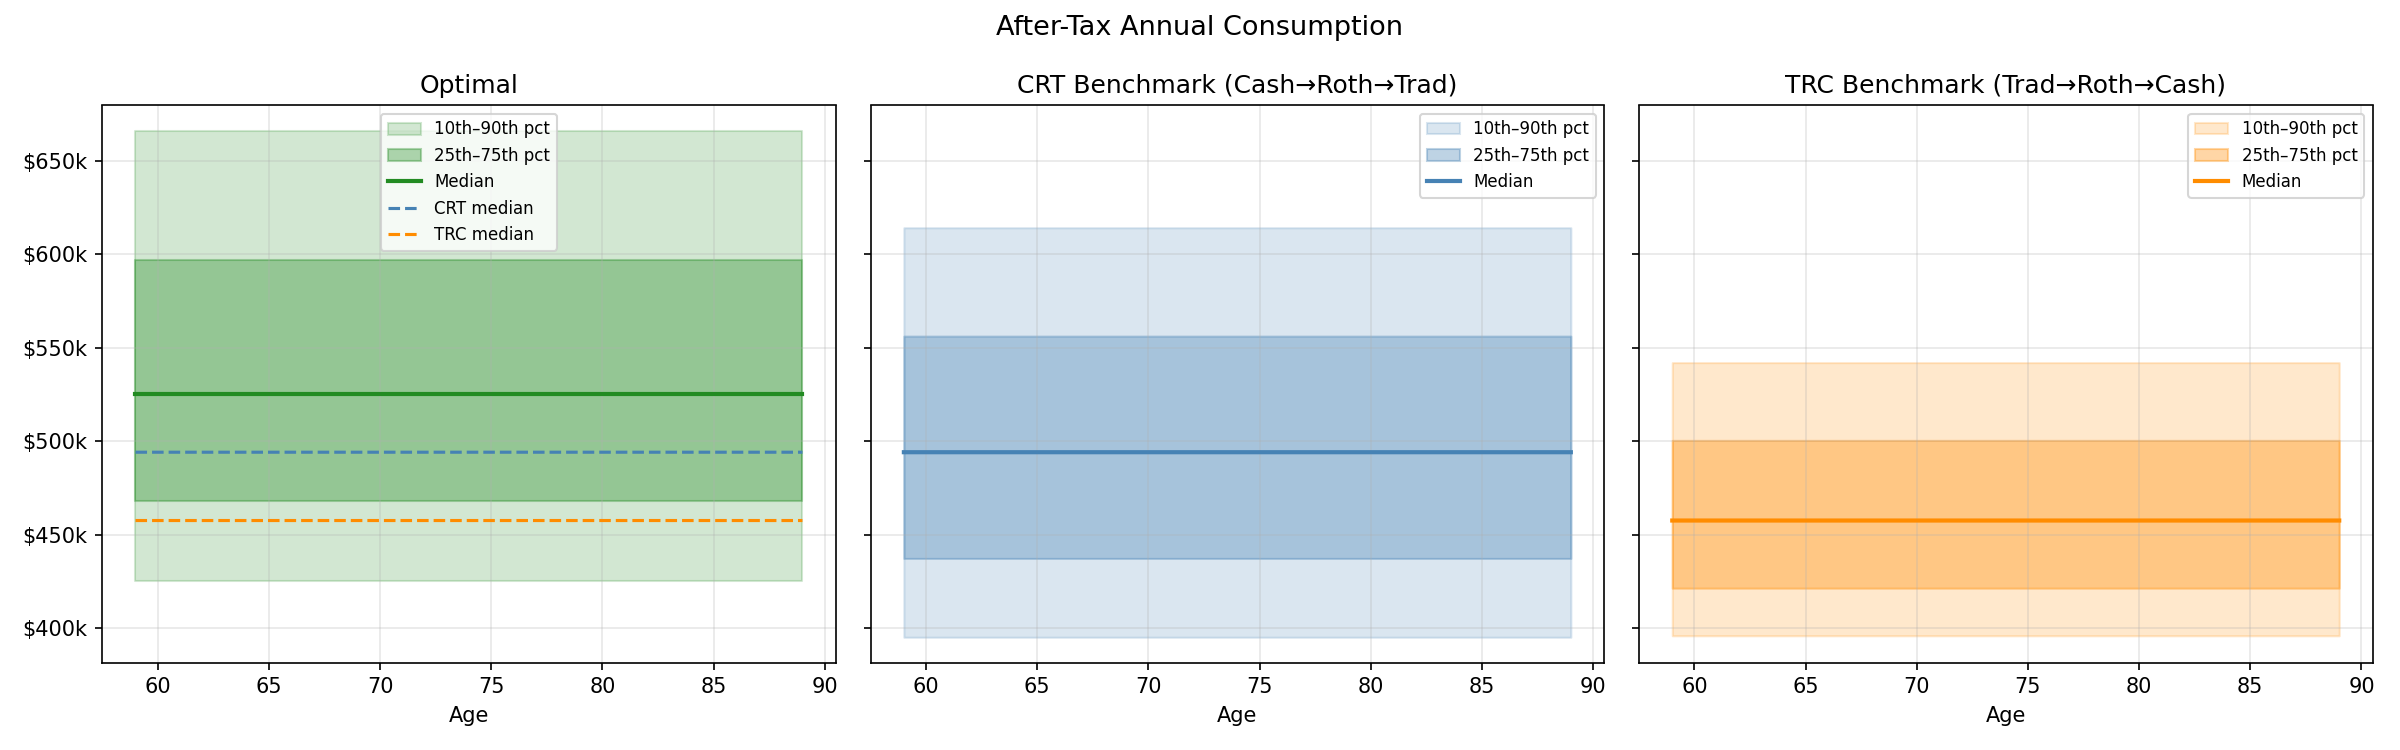
\includegraphics[width=\textwidth]{../plots/consumption.png}
  \caption{After-tax annual consumption: optimizer (left), muni-first
           benchmark $\Cmdr$ (center), deferred-first benchmark $\Cdrm$ (right).
           Bands show 10th--90th and 25th--75th percentiles across 1,000 simulations;
           the solid line is the median. Dotted lines in the left panel overlay the
           benchmark medians for reference.}
  \label{fig:consumption}
\end{figure}

\subsection{Tax Outcomes}

Table~\ref{tab:taxes} reports the cross-simulation distribution of lifetime
federal income taxes.

\begin{table}[h]
\centering
\caption{Distribution of Lifetime Federal Income Taxes Across 1,000 Simulations (\$)}
\label{tab:taxes}
\begin{tabular}{@{} lrrrrrr @{}}
\toprule
& \textbf{P10} & \textbf{P25} & \textbf{Median} & \textbf{Mean} & \textbf{P75} & \textbf{P90} \\
\midrule
Lifetime taxes & 462,802 & 504,819 & 560,429 & 575,430 & 630,523 & 701,891 \\
\bottomrule
\end{tabular}
\end{table}

Median lifetime taxes are \$560,429 over 33 years, or roughly \$17,000 per
year on median constant consumption of \$258,249 --- an effective lifetime rate
of approximately 6.6\%. The P90/P10 spread of \$239,089 is driven by variation
in stock returns: stronger equity performance inflates the traditional IRA
balance and forces larger taxable withdrawals, generating higher taxes even
under an optimal withdrawal policy. This cross-simulation variance is
irreducible, reflecting the fundamental link between portfolio outcomes and
tax obligations in a tax-deferred account.

Figure~\ref{fig:marginal} shows the distribution of effective marginal tax
rates by age. The optimizer consistently keeps most paths in the 12--22\%
brackets throughout the horizon, avoiding the 24\%+ brackets by moderating
traditional IRA withdrawals in years when Social Security is also included
in taxable income.

\begin{figure}[h]
  \centering
  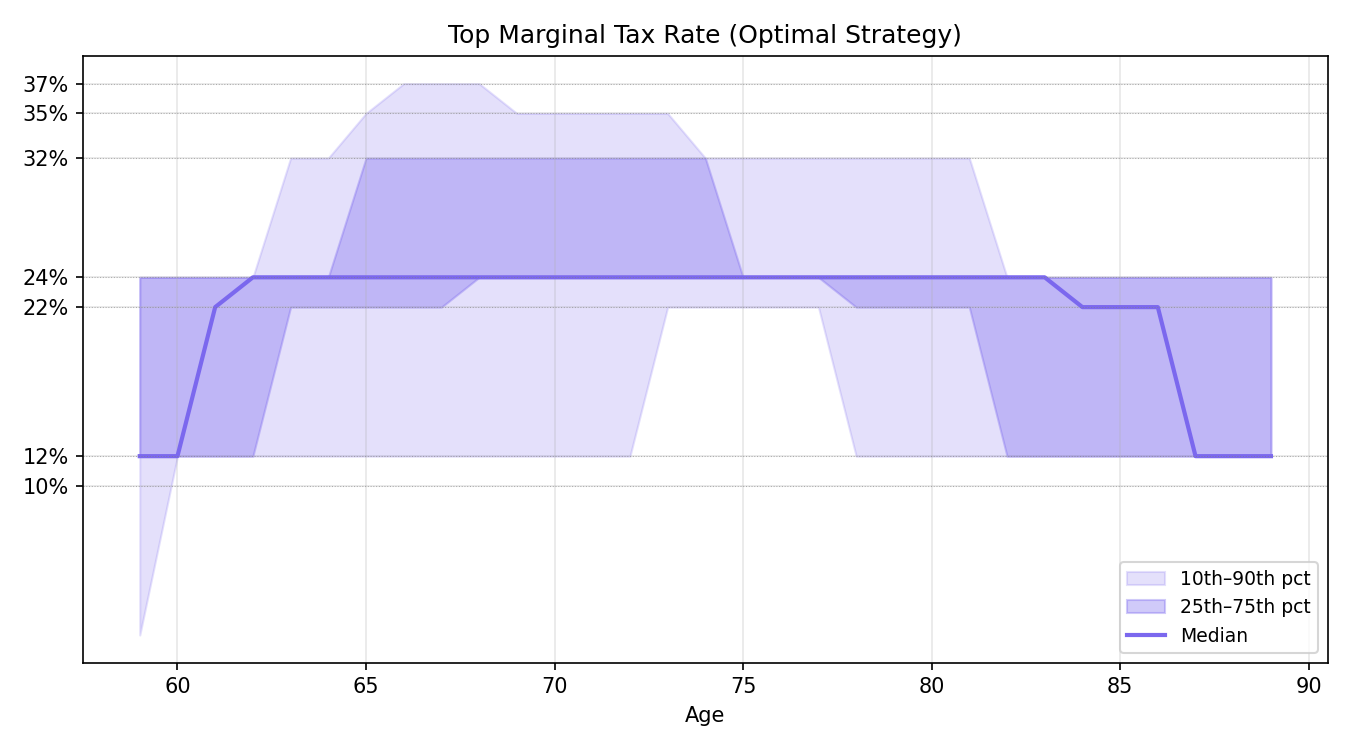
\includegraphics[width=0.78\textwidth]{../plots/marginal_rates.png}
  \caption{Distribution of marginal federal tax rates by age across 1,000 simulations.}
  \label{fig:marginal}
\end{figure}

\begin{figure}[h]
  \centering
  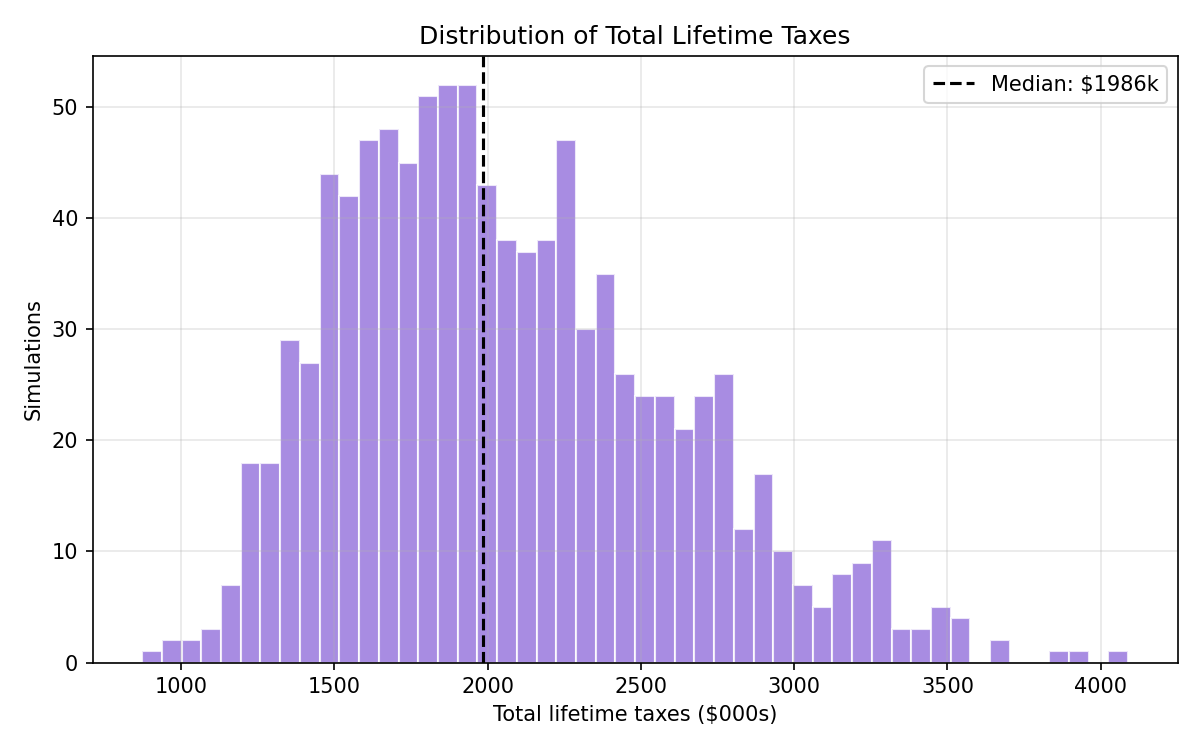
\includegraphics[width=0.65\textwidth]{../plots/tax_dist.png}
  \caption{Cross-simulation distribution of lifetime federal income taxes.}
  \label{fig:taxes_fig}
\end{figure}

\subsection{Account Drawdown Paths}

Figure~\ref{fig:balances} shows the median and interquartile range of each
account balance over the planning horizon; Figure~\ref{fig:withdrawals} shows
the corresponding annual withdrawals.

\begin{figure}[h]
  \centering
  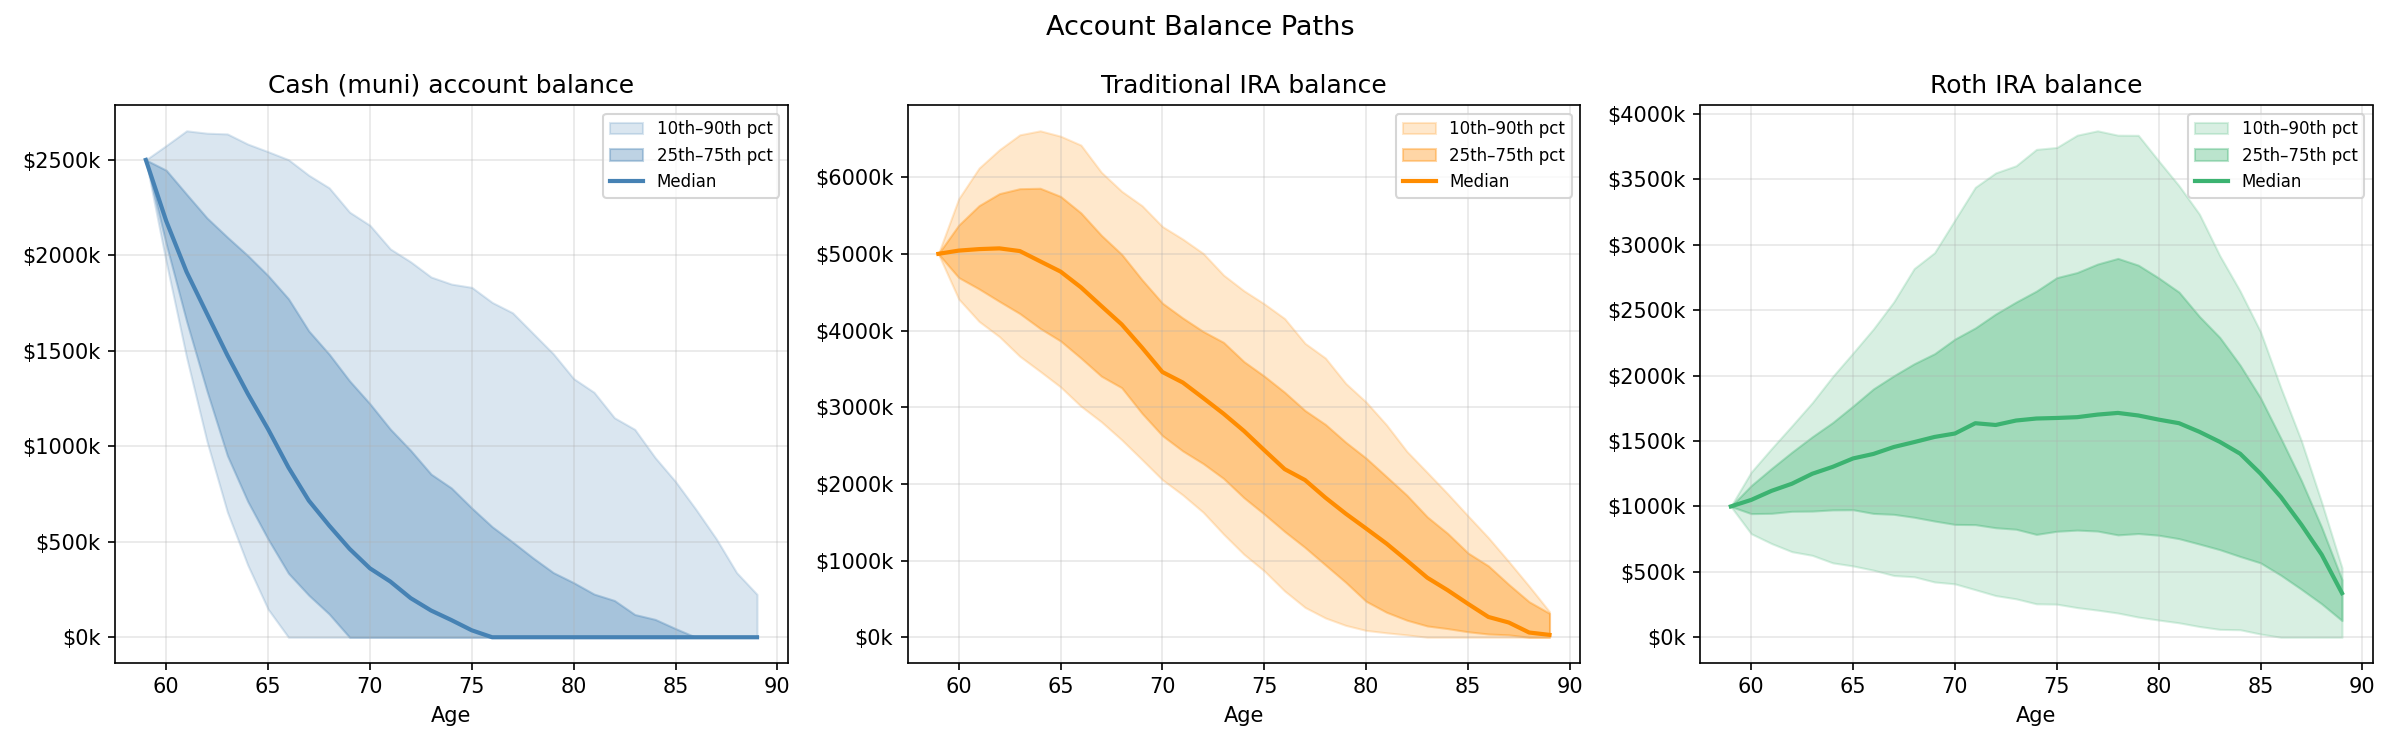
\includegraphics[width=\textwidth]{../plots/balances.png}
  \caption{Account balances by age: muni-bond account (left), traditional IRA
           (center), Roth IRA (right). Bands show 10th--90th and 25th--75th
           percentiles; solid line is the median.}
  \label{fig:balances}
\end{figure}

\begin{figure}[h]
  \centering
  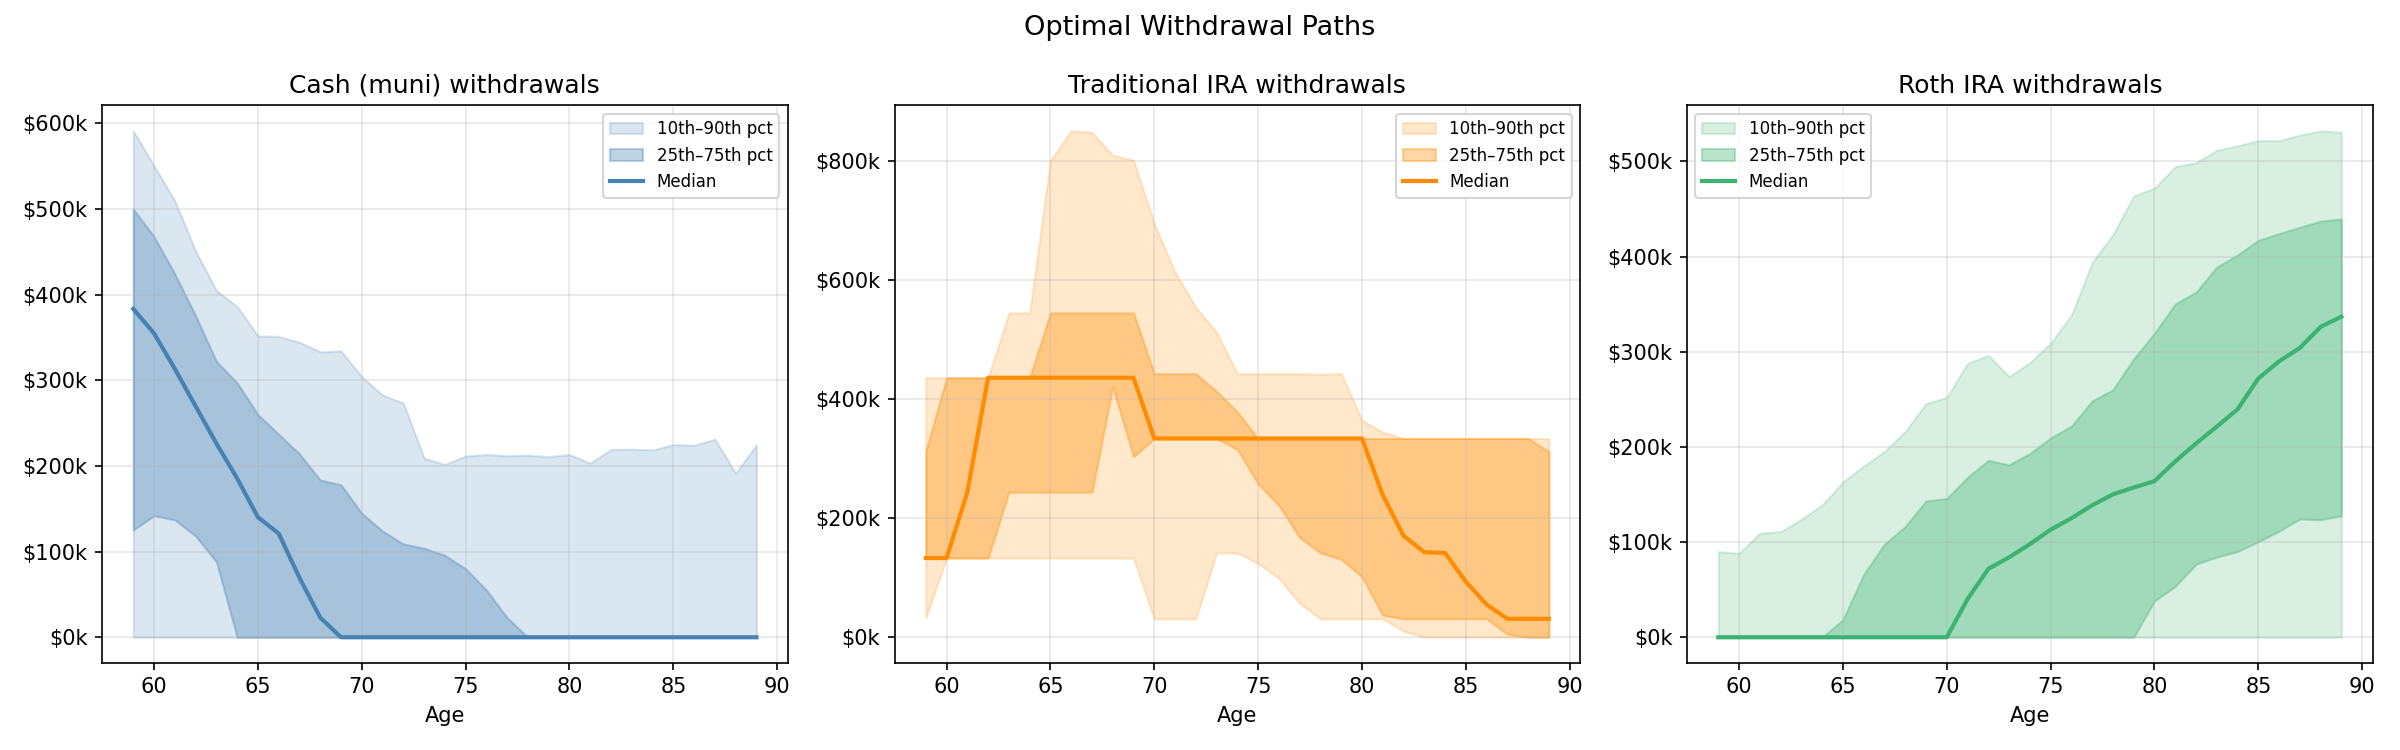
\includegraphics[width=\textwidth]{../plots/withdrawals.png}
  \caption{Annual withdrawals by account type. Muni and Roth withdrawals are
           tax-free; traditional IRA withdrawals constitute ordinary income.}
  \label{fig:withdrawals}
\end{figure}

Several patterns are visible. First, the traditional IRA is drawn down
substantially in the pre-Social Security years (ages 59--69), when the sole
source of taxable income is $w^d_t$ itself and the marginal rate is relatively
low. As Social Security begins at age 70 and adds \$102,000 to taxable income,
traditional IRA withdrawals fall and the remaining traditional IRA balance is
primarily liquidated through RMDs. Second, the muni account serves as a bridge,
supplementing traditional IRA income before Social Security begins. Third, the
Roth account is drawn down later, once the other tax-free muni source is
exhausted.

On high-return paths, the Roth account retains a small positive balance at
death (median terminal Roth $\approx \$140{,}000$). As discussed in
Remark~\ref{rem:terminal}, this reflects the constraint that Social Security
income in later years already covers most of $\Copt$, leaving limited capacity
to draw additional tax-free income from the Roth without simply accepting that
it will not be fully depleted.

% =============================================================================
\section{Conclusion}
\label{sec:conclusion}

We have developed and implemented a Monte Carlo--LP framework for optimizing
retirement account withdrawals across three account types with distinct tax
treatments. The core observation is that, for a given realized sequence of
stock returns, the constant-consumption withdrawal problem is a Linear Program
with roughly 300 variables and 600 constraints, solvable in milliseconds. A
Monte Carlo wrapper over 1,000 independent return paths yields a complete
distributional picture of sustainable consumption and lifetime taxes.

Under our baseline calibration --- \$3.5 million in initial wealth,
\$120,000 in annual Social Security benefits, and historical equity return
parameters --- the optimizer supports a median constant after-tax consumption
of \$258,249 per year, roughly 7\% above simple account-priority heuristics.
Lifetime federal taxes are held to a median of \$560,000 over 33 years, with
effective marginal rates concentrated in the 12--22\% range throughout the
horizon.

Several extensions are natural and left for future work. First, the Social
Security claiming age $a_{SS}$ is treated as fixed; an outer optimization
over $a_{SS}$ could find the claiming age that maximizes expected $\Copt$.
Second, the model could incorporate state income taxes, which vary
significantly across states and affect the relative attractiveness of muni
versus traditional IRA withdrawals. Third, the planning horizon $a_\dagger$
could be treated as stochastic, integrating over a mortality distribution
rather than conditioning on a fixed death age. Fourth, Roth conversion
strategies --- transferring funds from the traditional IRA to the Roth prior
to RMD age to reduce future taxable distributions --- could be incorporated
as an additional set of decision variables.

% =============================================================================
\clearpage
\appendix

% =============================================================================
\section{Complete LP in Standard Form}
\label{app:lp}

We index the decision variables as follows. Let $T$ be the horizon length and
$K = 7$ the number of tax brackets. Define index functions
\begin{align*}
  i_m(t)   &= t,              &    &t = 0,\ldots,T-1, \\
  i_d(t)   &= T + t,          &    &t = 0,\ldots,T-1, \\
  i_r(t)   &= 2T + t,         &    &t = 0,\ldots,T-1, \\
  i_s(t,k) &= 3T + tK + k,   &    &t = 0,\ldots,T-1,\; k=0,\ldots,K-1, \\
  i_C      &= 3T + TK.        &    &\text{(scalar } \Copt\text{)}
\end{align*}
The total number of variables is $N + 1 = 3T + TK + 1$.
Let $\mathbf{x} \in \mathbb{R}^{N+1}$ collect all variables.

\subsubsection*{Objective vector}
$\mathbf{c} \in \mathbb{R}^{N+1}$: all entries zero except $c_{i_C} = -1$.

\subsubsection*{Equality constraints}
One row per year $t = 0, \ldots, T-1$, enforcing constant after-tax consumption:
\[
  x_{i_m(t)} + (1-\pi_t)\,x_{i_d(t)} + x_{i_r(t)}
  - \sum_{k=0}^{K-1} \Delta\tau_k\, x_{i_s(t,k)}
  - x_{i_C}
  \;=\; -y^{SS}_t - y^{emp}_t - y^{pen}_t.
\]
The coefficient $(1-\pi_t)$ on $x_{i_d(t)}$ incorporates the early
withdrawal penalty~\eqref{eq:penalty_rate}; $\pi_t = 0$ for all years
in which the planner is age $59\tfrac{1}{2}$ or older.

\subsubsection*{Inequality constraints}
All inequalities are of the form $\mathbf{A}_{\mathrm{ub}}\,\mathbf{x} \leq \mathbf{b}_{\mathrm{ub}}$.

\smallskip
\textit{(a) Tax bracket slacks} ($TK$ rows):
\[
  x_{i_d(t)} - x_{i_s(t,k)} \;\leq\; \Delta + L_k - \phi\,y^{SS}_t - y^{emp}_t - y^{pen}_t,
  \quad t = 0,\ldots,T-1,\; k = 0,\ldots,K-1.
\]

\textit{(b) Muni-account non-negativity} ($T$ rows, for $t = 1, \ldots, T$):
\[
  \sum_{\tau=0}^{t-1} \frac{G^m_t}{G^m_\tau}\,x_{i_m(\tau)}
  \;\leq\; A^m_0\,G^m_t.
\]

\textit{(c) Traditional IRA non-negativity} ($T$ rows):
\[
  \sum_{\tau=0}^{t-1} \frac{G^d_t}{G^d_\tau}\,x_{i_d(\tau)}
  \;\leq\; A^d_0\,G^d_t.
\]

\textit{(d) Roth non-negativity} ($T$ rows):
\[
  \sum_{\tau=0}^{t-1} \frac{G^r_t}{G^r_\tau}\,x_{i_r(\tau)}
  \;\leq\; A^r_0\,G^r_t.
\]

\textit{(e) RMD constraints} (one row per $t$ with $a_0 + t \geq a_{\mathrm{RMD}}$):
\[
  -\nu_t\,x_{i_d(t)}
  - \sum_{\tau=0}^{t-1} \frac{G^d_t}{G^d_\tau}\,x_{i_d(\tau)}
  \;\leq\; -A^d_0\,G^d_t.
\]

\subsubsection*{Variable bounds}
\[
  x_{i_m(t)},\; x_{i_d(t)},\; x_{i_r(t)},\; x_{i_s(t,k)} \;\geq\; 0;
  \qquad x_{i_C} \in \mathbb{R} \;\text{(unrestricted)}.
\]

% =============================================================================
\section{2026 Federal Income Tax Schedule (Married Filing Jointly)}
\label{app:tax}

\begin{table}[h]
\centering
\caption{2026 Married Filing Jointly Tax Brackets}
\label{tab:brackets}
\begin{tabular}{@{} R{3cm} R{3cm} C{3cm} @{}}
\toprule
\textbf{Taxable income: from} & \textbf{to} & \textbf{Marginal rate} \\
\midrule
\$0          & \$24,800    & 10\% \\
\$24,800     & \$100,800   & 12\% \\
\$100,800    & \$211,400   & 22\% \\
\$211,400    & \$403,550   & 24\% \\
\$403,550    & \$512,450   & 32\% \\
\$512,450    & \$768,700   & 35\% \\
\$768,700    & $\infty$    & 37\% \\
\midrule
\multicolumn{2}{@{}l}{Standard deduction (MFJ 2026)} & \$32,200 \\
\bottomrule
\end{tabular}
\end{table}

\noindent
Taxable income is ordinary income $I_t$ less the standard deduction:
$\max(0,\, I_t - \$32{,}200)$. The tax function implemented in the optimizer
is $\Tax(I) = \sum_k \Delta\tau_k \cdot \max(0, I - \Delta - L_k)$,
where the bracket increments are $\Delta\tau_0 = 10\%$,
$\Delta\tau_1 = 2\%$, $\Delta\tau_2 = 10\%$, $\Delta\tau_3 = 2\%$,
$\Delta\tau_4 = 8\%$, $\Delta\tau_5 = 3\%$, $\Delta\tau_6 = 2\%$.

% =============================================================================
\section{IRS Uniform Lifetime Table (Selected Ages)}
\label{app:rmd}

The distribution period $\nu_t$ in the RMD calculation is taken from the IRS
Uniform Lifetime Table (Rev.\ Proc.\ 2022-32). This table applies to unmarried
owners and to married owners whose spouse is not more than 10 years younger.
The full table used in the optimizer covers ages 60 through 120.

\begin{table}[h]
\centering
\caption{IRS Uniform Lifetime Table: Selected Ages}
\label{tab:rmd}
\begin{tabular}{@{} C{2.5cm} C{3.5cm} @{}}
\toprule
\textbf{Age} & \textbf{Distribution period $\nu$} \\
\midrule
73 & 26.5 \\
74 & 25.5 \\
75 & 24.6 \\
76 & 23.7 \\
77 & 22.9 \\
78 & 22.0 \\
79 & 21.1 \\
80 & 20.2 \\
85 & 16.0 \\
90 & 12.2 \\
95 &  8.9 \\
\bottomrule
\end{tabular}
\end{table}

\noindent
The required minimum distribution for a given year is $\rho_t = A^d_t / \nu_t$.
At age 73 this requires distributing approximately 3.8\% of the account balance;
by age 90 the required fraction exceeds 8\%.

\end{document}
